\documentclass{article}
\usepackage[a4paper,left=3cm,right=3cm,top=3cm,bottom=3cm]{geometry}
\usepackage[utf8]{inputenc}
\usepackage[T1]{fontenc}
\usepackage{latexsym,amsfonts,amsmath,amssymb,amstext,graphicx,titlesec,ae,aecompl,mathtools,tabularx, multirow, cancel, nicefrac,subcaption, blindtext, floatrow}
\setlength{\parindent}{0pt}
\newfloatcommand{capbtabbox}{table}[][\FBwidth]


\begin{document}

\begin{titlepage}
       \begin{center}
             \begin{huge}
				   %% Update assignment number here
                   \textbf{Assignment 2}
             \end{huge}
       \end{center}

       \begin{center}
             \begin{large}
                   Computational Intelligence, SS2020
             \end{large}
       \end{center}

       \begin{center}
 \begin{tabularx}{\textwidth}{|>{\hsize=.33\hsize}X|>{\hsize=.33\hsize}X|>{\hsize=.33\hsize}X|} 

                   \hline
                   \multicolumn{3}{|c|}{\textbf{Team Members}} \\
                   \hline
                   Last name & First name & Matriculation Number \\
                   \hline
                   Blöcher & Christian & 01573246 \\
                   \hline
                   Bürgener & Max & 01531577 \\
                   \hline
                    &  &  \\
                   \hline

             \end{tabularx}
       \end{center}
\end{titlepage}

\section{Linear regression}

\subsection{Derivation of Regularized Linear Regression}

\begin{itemize}

%    \begin{figure}[h]
%        \centering
%        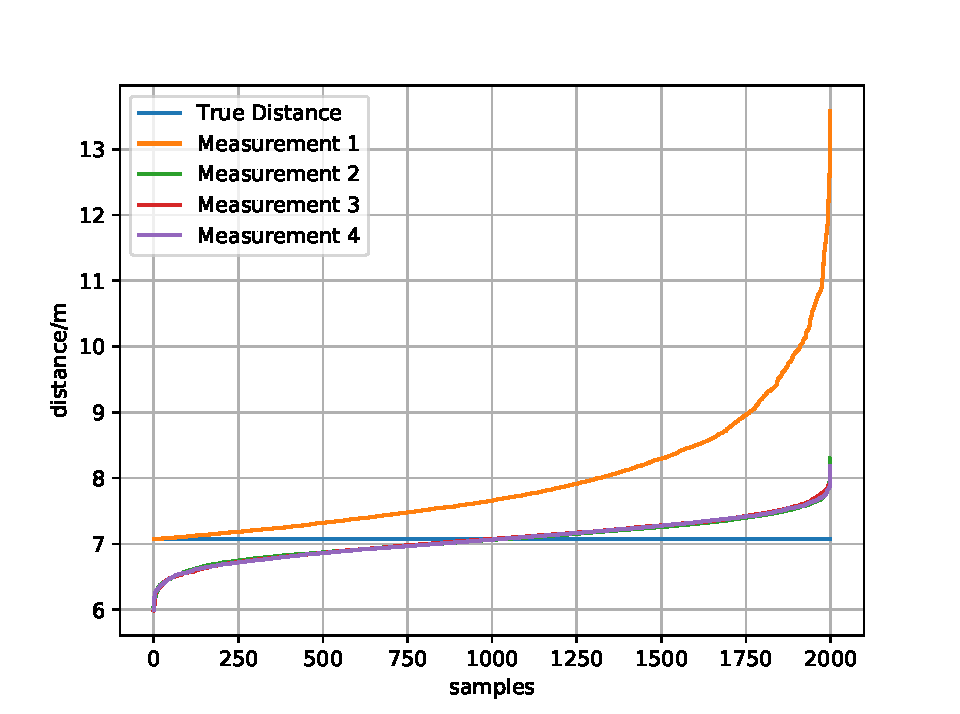
\includegraphics[width=\textwidth]{./Figures/scenario2_findexponential.pdf}
%        \caption{Scenario 2 with mixed measurement models for the anchors}
%        \label{fig:scenario2_findexponential}
%    \end{figure}
    
    \item Why is the design matrix $\boldsymbol{X}$ containing $n + 1$ and not just $n$?
    
    \begin{itemize} 
    
        \item The simplest form of linear regression is calculated by:
            $$y(\boldsymbol{x, \omega}) = \underset{bias}{\underbrace{\omega_0}} + \boldsymbol{\omega}^T \boldsymbol{w}$$
        \item The additional column is used to compensate the sum of the bias $\omega_0$ and thus to simplify our calculation. \\
      
            $$ \boldsymbol{X} = 
            \begin{bmatrix}
	            1		& \dots		& x_1	\\
	            \vdots	& \ddots 	& \vdots		\\
	            1		& \dots 		& x_N
	            \end{bmatrix}
	            \begin{bmatrix}
	            \omega_0 \\
	            \vdots	 \\
	            \omega_N	 
            \end{bmatrix} $$
     \end{itemize}
    
    \item What is the dimension of the gradient vector?
    
    \begin{itemize}
        \item The gradient contains the derivation of all $J\boldsymbol{(\theta)}$ for all variables. That means the gradient has the dimension $m \times 1$ and it contains a group of targets. \\        
            $$\frac{\partial J(\boldsymbol{\boldsymbol{\theta)}}}{\partial \boldsymbol{\theta}} =
            \begin{bmatrix}
            	\frac{\partial J(\boldsymbol{\theta)}}{\partial \theta_1}	 \\
            	\vdots \\
            	\frac{\partial J(\boldsymbol{\theta)}}{\partial \theta_m}  	
            \end{bmatrix}$$     
    \end{itemize} 
    
    \item What is the definition of the Jacobian matrix and what is the difference between the gradient and the Jacobian matrix?
    
    \begin{itemize}
        \item The Jacobian matrix elements are calculated by the derivatives of all outputs of a vector with respect to all parameters.  \\
            $$ \boldsymbol{J} = 
            \begin{bmatrix}
            	\frac{\partial y_1}{\partial x_1}	&	\dots	&	\frac{\partial y_1}{\partial x_n} 	\\
            	\vdots								&	\ddots	&	\vdots								\\
            	\frac{\partial y_m}{\partial x_1	}	&	\dots	&	\frac{\partial y_m}{\partial x_n}
            \end{bmatrix} $$
            
        \item The gradient is computed from a scalar. It is a vector which contains the derivatives of a function for all parameters.              
    \end{itemize}
    
    \item What is the dimension of the Jacobian matrix and what is it equal to?
    
    \begin{itemize}
    
        \item The dimension of the Jacobian matrix equals the dimension of the Design matrix
    
    \end{itemize}
    
    \item Minimization of the regularized linear regression cost function
    
    $$\begin{array}{rclr}
        J(\boldsymbol{\theta}) & = & \frac{1}{m} \| \boldsymbol{X\theta - y} \|^2 + \frac{\lambda}{m} \| \boldsymbol{\theta}^2 \| & \\\\
        J(\boldsymbol{\theta}) & = & \frac{1}{m} \left[(\boldsymbol{X\theta - y})^T \cdot (\boldsymbol{X\theta - y}) \right] + \frac{\lambda}{m} (\boldsymbol{\theta^T \theta}) & \mid \frac{\partial}{\partial\boldsymbol{\theta}} \\
    \end{array}$$
    
    Using Hint 2 from our exercise sheet the calculation is simplified to:
    
    $$\begin{array}{rclr}
        \frac{\partial J(\boldsymbol{\theta})}{\partial \boldsymbol{\theta}} & = & \frac{2}{m}(\boldsymbol{X\theta - y})^T \cdot \boldsymbol{X} + \frac{2\lambda}{m}\ \boldsymbol{\theta}^T & \mid \overset{!}{=} 0
    \end{array}$$

    We set the gradient to zero to calculate our solution $\theta$
    
    $$\begin{array}{rclr}    
    \frac{2}{m}(\boldsymbol{\theta}^T \boldsymbol{X}^T \boldsymbol{X} - \boldsymbol{y}^T \boldsymbol{X}) + \frac{2\lambda}{m}\boldsymbol{\theta}^T & = & 0 \\\\
    \boldsymbol{\theta}^T \boldsymbol{X}^T \boldsymbol{X} + \lambda \boldsymbol{\theta}^T & = & \boldsymbol{y}^T \boldsymbol{X} & \\\\
    \boldsymbol{\theta}^T (\boldsymbol{X}^T \boldsymbol{X} + \lambda E) & = & \boldsymbol{y}^T\boldsymbol{X} & \\\\
    \boldsymbol{\theta}^T & = & (\boldsymbol{y}^T \boldsymbol{X})(\boldsymbol{X}^T \boldsymbol{X} + \lambda \boldsymbol{E})^{-1} & \mid ()^T \\\\
    \end{array}$$
	
	Due to the property of transpose: $ (\boldsymbol{A}\boldsymbol{B})^T = \boldsymbol{B}^T\boldsymbol{A}^T $ we get:
	
	$$\begin{array}{rcl}
	
    \theta & = & (\boldsymbol{X}^T\boldsymbol{X} + \lambda\boldsymbol{E})^{-1^T} (\boldsymbol{y}^T\boldsymbol{X})^T \\\\
    \theta & = & (\boldsymbol{X}^T\boldsymbol{X} + \lambda\boldsymbol{E})^{-1} (\boldsymbol{X}^T\boldsymbol{y})
	\end{array}$$

    
    
    
 
    
\end{itemize}

\subsection{Linear Regression with polynomial features}


\subsection{(Bonus) Linear Regression with radial basis functions}


\section{Logistic Regression}

\subsection{Derivation of Gradient}

\subsection{Logistic Regression training with gradient descent}

\end{document}